\documentclass[12pt]{article}

\usepackage{fullpage,amsmath,amssymb,setspace,graphicx}

\newtheorem{remark}{Remark}
             
\newcommand{\ignore}[1]{}
             
% SPACING    
\newcommand{\vcm}[1][1]{\vspace*{#1 cm}}
\newcommand{\hcm}[1][1]{\hspace*{#1 cm}}
\newcommand{\rb}[2]{\raisebox{#1 mm}[0mm][0mm]{#2}}
\newcommand{\istrut}[2][0]{\rule[- #1 mm]{0mm}{#1 mm}\rule{0mm}{#2 mm}}
\newcommand{\zeromath}[1]{\makebox[0mm][l]{$#1$}}
\newcommand{\zero}[1]{\makebox[0mm][r]{#1}}

% MATH
\newcommand{\E}{{\mathbb E\/}}
\newcommand{\paren}[1]{{\left( #1 \right)}}
\newcommand{\bigparen}[1]{\big( #1 \big)}
\newcommand{\biggparen}[1]{\bigg( #1 \bigg)}
\newcommand{\angbrack}[1]{\left< #1 \right>}
\newcommand{\Angbrack}[1]{\Big< #1 \Big>}
\newcommand{\curlybrack}[1]{\left\{ #1 \right\}}
\newcommand{\bigcurly}[1]{\big\{ #1 \big\}}
\newcommand{\biggcurly}[1]{\bigg\{ #1 \big\}}
\newcommand{\sqbrack}[1]{\left[ #1 \right]}
\newcommand{\SqBrack}[1]{\Big[ #1 \Big]}
\newcommand{\SQBrack}[1]{\bigg[ #1 \bigg]}
\newcommand{\Paren}[1]{\Big( #1 \Big)}
\newcommand{\PAREN}[1]{\bigg( #1 \bigg)}
\newcommand{\abs}[1]{\left| #1 \right|}
\newcommand{\ceil}[1]{\left\lceil #1 \right\rceil}
\newcommand{\floor}[1]{\lfloor #1 \rfloor}
\newcommand{\f}[2]{\frac{#1}{#2}}
\newcommand{\fr}[2]{\mbox{$\frac{#1}{#2}$}}
\newcommand{\modulo}{ {\mbox{ \rm mod } }}
\newcommand{\logstar}{{\log^*}}
\newcommand{\bydef}{\stackrel{\operatorname{def}}{=}}
\newcommand{\poly}{\operatorname{poly}}
\newcommand{\polylog}{\operatorname{polylog}}
\newcommand{\bottom}{\perp}
\newcommand{\dist}{\operatorname{dist}}
\newcommand{\argmin}{\operatornamewithlimits{argmin}}

\linespread{1.5}
\begin{document}


{\bf Understanding the effect of coronavirus pandemic on 2020 US presidential election across counties} \\

{\bf Introduction}

 The 2020 US presidential election has come to an end with Joe Biden winning 306 electoral votes, yet the year of 2020 has been special with the spread of coronavirus pandemic across the world. USA is so far the most affected country with 11.4 million confirmed cases and 248000 deaths as of November 18, 2020. The mortality rate is $2.2\%$, lower than the global average rate $2.4 \%$. The pandemic spreads more rapidly in urban area with higher population density, and the variance in confirmed cases, deaths and mortality is large across states and counties.
  
 Some people and experts blame Trump administration for the country's failure to contain the outbreak. Over the past months, he understated the dangers posed by the virus, belittled masks and social-distancing requirements, suppressed scientists working to study the virus etc. Our primary interest of the paper is to quantify the effect of coronavirus (covid-19) on the result of the 2020 presidential election at the county-level based on techniques such as regression and bootstrapping. More specifically, we would like to answer questions such as how confirmed cases, deaths per 1 million population and case fatality rate affected the vote share of Donald Trump while controlling other socio-economic variables?
 
 There are numerous papers analyzing the voting behavior of the 2016 presidential election. Scala and Johnson (2017) examined how race, religion, income and education are related to Trump's vote shares, and claimed in 2016 Clinton faced increasingly difficult political climates on the rural side of the urban-rural interface. According to  Goldman, Lim, Chen et al (2018), the net Republican gain in 2016 was greater in rural counties with higher age-adjusted death rates. Similarly, Shannon M. Monnat showed Trump over-performed the most counties with the highest drug, alcohol and suicide mortality rates. Stoetzer, Gerlich and Koesters (2017) found that counties with a larger proportion of white Americans, low education and income, high unemployment rate tend to vote for Trump, and the state fixed effect is the most relevant factor.
 
 
 We will focus on the effect of coronavirus pandemic on the vote shares of Trump, but inspired by previous researches, we will also have socio-economic factors in the model. The socio-economic variables, on the one hand contribute to the accuracy of the model, on the other hand, are likely to be confounders that we have to control in order to precisely quantify the net effect of covid-19 on election results. Recent researches have supported that socio-economic status is correlated to coronavirus disease. For example, Hawkins, Charles and Mehaffey (2020) showed at county-level, education, proportion of black residents and poverty rate are all associated with covid-19 cases and fatalities.  Nivedita Mukherji (2020) illustrated that counties with high median income have a high incidence of cases but reported lower deaths.
 
 In the next sections of the paper, we will introduce how the data were collected from various sources and present the methods to be used. We will present a multivariate linear regression model, estimate its confidence interval with different methods, and use bootstrapping to estimate the vote share of Trump under imaginary scenarios.  \\
 
 
 ... (might have modifications) \\
 
 {\bf Data}
 
 We collected most socio-economic data from the U.S. Census Bureau, including total area and race information of each county from 2010 census, population in 2019, and poverty rate (from the Small Area Income and Poverty Estimates Program of the Bureau), education and median household income in 2018. The county-level unemployment rates in 2019 are from Local Area Unemployment Statistics  program of the Bureau of Labor Statistics .
 
 The coronavirus data at county-level, consisting of confirmed cases and deaths are from USAFacts (USAFacts(2020). Known cases, deaths. Retrieved from https://usafacts.org/
 visualizations/
 coronavirus-covid-19-spread-map/), which is a nonpartisan civic initiative making government data available for all. We included the cumulative confirmed cases and deaths up to the end of October in our dataset. The 2020 presidential election results are from Thomson Reuters, loaded and transformed from web service and made available on Kaggle by Raphael Fontes. 
 
  We derived a few useful variables from the raw data. For each county, We first calculated the population density, and the number of cases/deaths per one thousand people. The case fatality rate is also included by dividing the number of total deaths by that of total cases. 
  
 
 There are 3141 counties in total in the US, and after removing counties with missing values, we have 2852 observations left in the dataset. Table 1 presents the median statistic for all the variables - the second and third ones are the summary statistics for counties that Trump won and Biden won respectively, of which the differcence is tested by Mood's median test.\\
 
 \begin{tabular}{cccc}
 	
 	\hline
 	Variable Name&  Biden won(n=427)& Trump won(n=2425)& P-value\\
 	\hline
 	Case fatality rate($\%$)& 2.08& 1.47& 0.000 \\
 	Total cases per 1k& 26.18& 24.85& 0.209 \\
 	Total deaths per 1k& 0.54& 0.36& 0.000\\
 	Population& 128990& 22195 &0.000\\
 	Population density(per square miles)& 157& 38& 0.000\\
 	High school education or less($\%$)& 21& 24.6& 0.000\\
 	Unemployment rate($\%$)& 3.8& 3.6& 0.145\\
 	Poverty rate($\%$)& 14.3& 14& 0.361\\
 	White population proportion($\%$)& 79.3& 94.1& 0.000\\
 	Black population proportion($\%$)& 8.9& 1.7& 0.000\\
 	Hispanic population proportion($\%$)& 5.6& 3.0& 0.000\\
 	Median household income(USD)& 56168& 49991& 0.000\\
    \hline
 	
 \end{tabular} \\
 
\centerline{ Table 1. Summary statistics of variables}

Without controlling for other variables like what we usually do in regression models, from Table 1 we can see Joe Biden tends to win in counties with denser population, higher education, higher proportion of black and hispanic population and higher median income. 

It is surprising that unemployment and poverty don't seem to be significant variables. One possible explanation is that these two rates are all from 2019, but the US unemployment rate soared to 14.7 percent in 2020 due to the impact of the pandemic. The most recent data should be more powerful in explaining the election results that the data from last year, but unfortunately we didn't find the data source for the  county-level unemployment data of 2020. Counties with higher unemployment or poverty rate in 2019 may still have the same tendency under the pandemic, but some industries are known to suffer the most, e.g. food, hospitality and transportation. People living in counties that reply heavily on the most affected industries, are more likely to lose jobs. 

The case fatality rate, total cases/deaths per one thousand people are all lower in counties where Trump won, however the difference in total cases isn't statistically significant. The virus spread faster in urban areas with denser population, and the supporters of Trump are, in contrast,  mostly from rural areas where the virus caused less trouble. If we control for confounding variables in the regression model, e.g. population density, the case fatality rate and total cases/deaths per 1k might become insignificant and the direction of their effect may even change. The significance of case fatality rate, and total cases per 1k will be our primary focus of the paper, and we will attempt to isolate their effect on the Trump's vote share by controlling the confounders in the model.

Figure 1 shows the pairwise correlation plot of several variables that are most correlated with each other in the dataset. The poverty rate is highly correlated with median household income, as expectated. It is also strongly correlated with education($r=0.65$), unemployment rate($r=0.52$) and white population proportion($r=-0.52$). Since we collected the poverty data from the Small Area Income and Poverty Estimates Program of US Census Bureau, it is likely that the poverty rate is estimated from socio-economic data by the program. Due to the collinearity we observed and the fact that poverty rate is not raw data from the census but inferred data, we will not use poverty rate for our further analysis.

The median household income is strongly correlated with education ($r=-0.54$) and unemployment rate($r=-0.43$) as expected.  It is also correlated ($r=0.30$) with population. Besides, the correlation coefficient between unemployment rate and education ($r=0.35$) and white population($r=-0.25$) proportion is moderate.


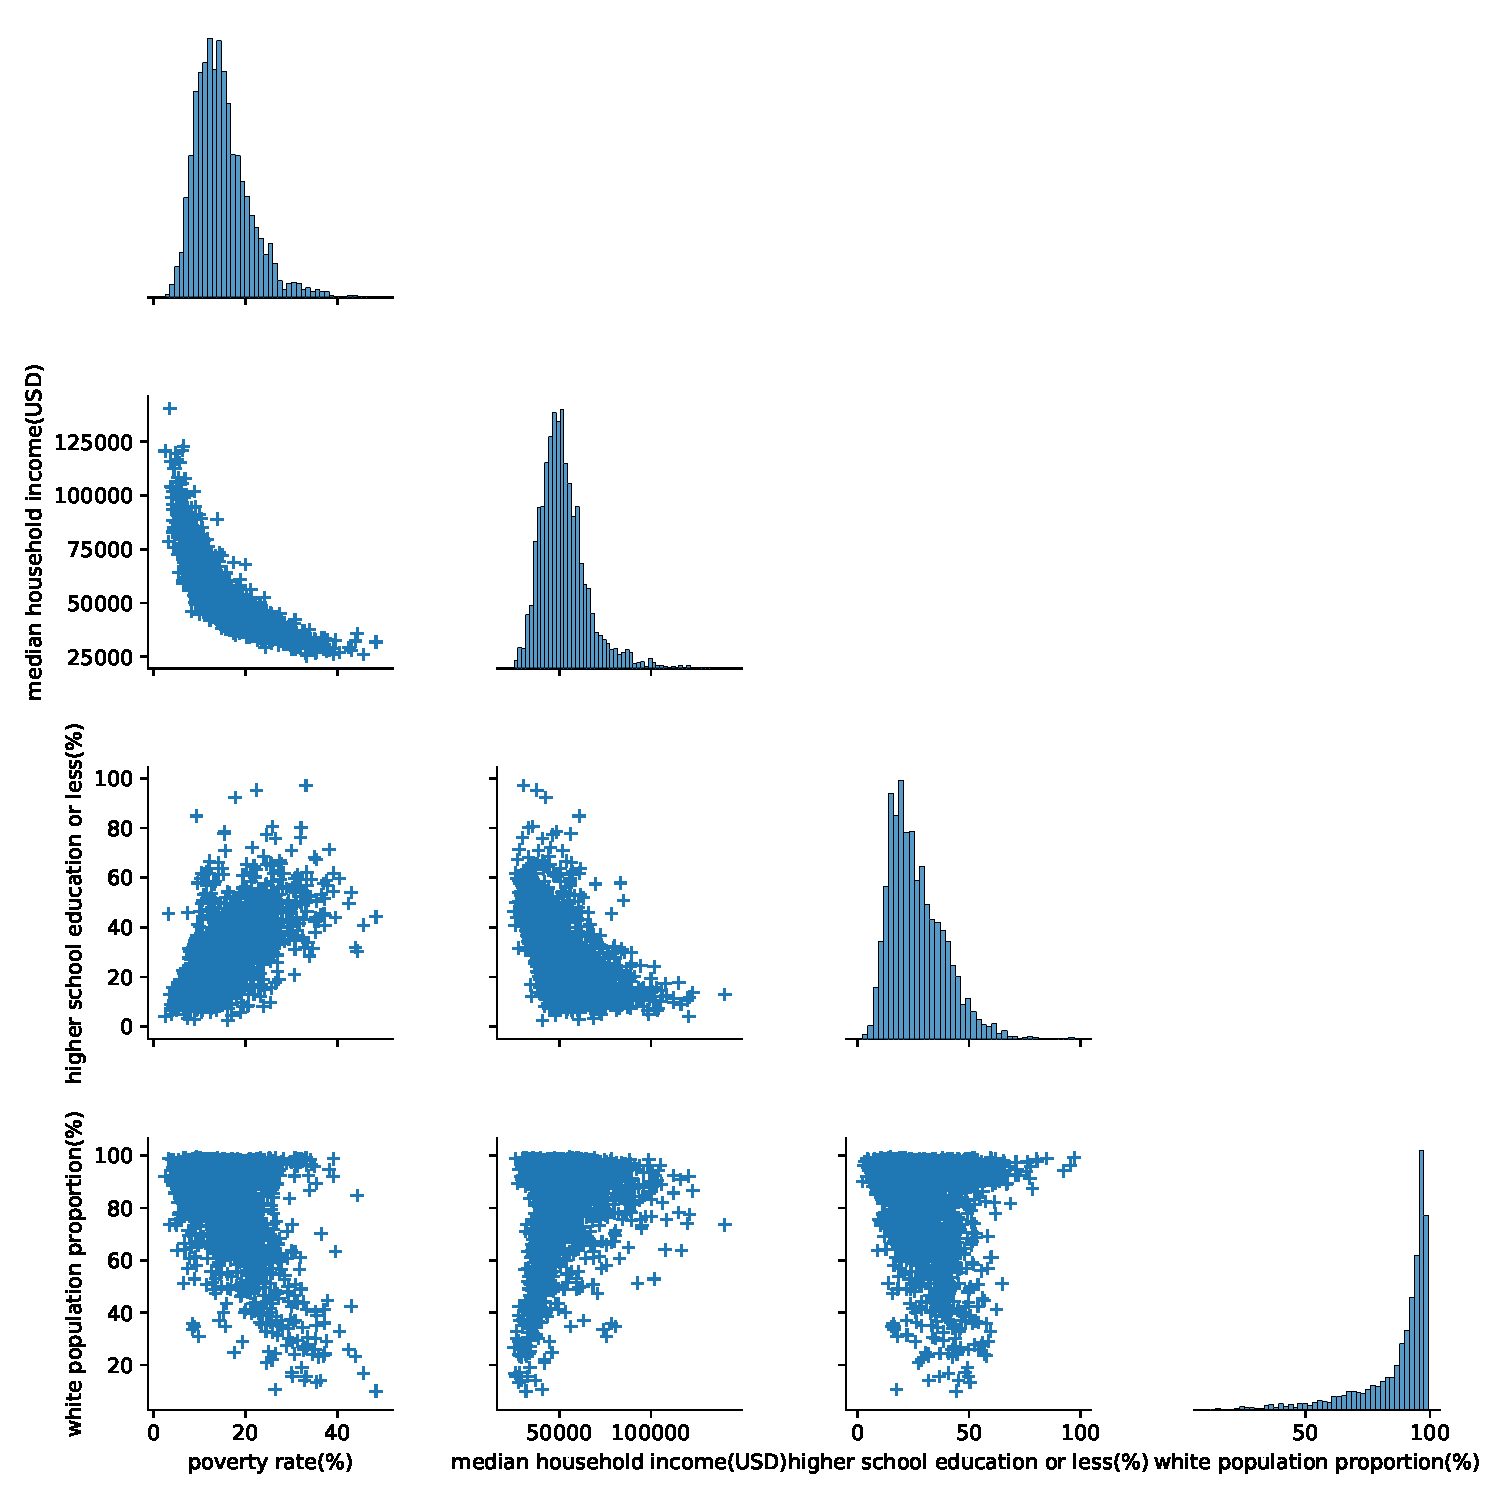
\includegraphics[scale=0.6]{cor_plot.pdf}

\centerline{ Figure 1. Pairwise correlation plot}


We didn't capture any interesting correlation (e.g. $r\geq0.2$) between case fatality rate and other variables. However, it appears that the total cases per one thousand people is moderately correlated with education ($r=0.37$) and the proportion of white population($r=-0.38$). Counties whose residents on average received less education tend to have more infections per one thousand, and in contrast, there are less cases for counties with a higher proportion of white population.\\


... (might have small modifications) \\

{\bf Method}

We will model the data with multivariate linear regression. The dependent variable will be Trump's vote share in percentage, we choose to use it instead of a binary variable indicating if Trump won the county or not, for the reason that vote share contains more information than a binary indicator. A win with $90\%$ vote share and another with $51\%$ shouldn't be treated equally.  With linear regression, we may worry about having predictions out of the range $[0,100]$, but for all the models we will analysis later on,  only in one model there is a single observation whose prediction falls below 0. A similar regression model with vote share as the outcome was also widely adopted by previous researches, such as Scala and Johnson (2017).  The base model is the following: \\

$ Vote\ Share\ of \ Trump=\beta_0 + {\bf\beta_1 State} + \beta_2 employment\_rate + \beta_3 median\_income +$  
$ \beta_3 education + \beta_4 population\_density + \beta_5 total\_cases\_per\_1k + \beta_6fatality\_rate + \beta_7population 
+ \beta_8 white\_population(\%) + \beta_9 hispanic\_population(\%) + \beta_{10} black\_population(\%) + \epsilon$ \\

To be clear about the notation, $State$ is for estimating the fixed effect of each state. In the model, we will transform it to dummy variables with Alabama as the baseline. In the later analysis, we will modify the above equation by adding interaction terms to our primary focus, which is total cases per 1k and case mortality rate. The goal is, on the one to hand quantify their effect on election result, on the other hand, to evaluate the heterogeneity of the effect across counties. The second goal can be achieved by accounting for interactions. The $\epsilon$ in the end of the model is what we called the error term, and we assume its mean is 0. The mean assumption suffices for the OLS estimates to unbiased, but further inferences based on student t test impose a normality assumption on it.  

To find the confidence intervals and p values, we will be using two methods - student t test and bootstrapping. The normality assumption may not hold in some cases, so we will also adopt the technique of bootstrapping. We will sample the original dataset with replacement for $5000$ times, and record the coefficients at each iteration. We will be able to have the distribution of all coefficient in the end of the bootstrapping, and the $95\%$ confidence interval extends from the $2.5\%$ percentile to the $97.5\%$ percentile (percentile interval). The p value is calculated exactly as how it is defined - the probability of obtaining test results as least as extreme as the results actually observed. A direct consequence is when the confidence interval excludes 0, we know immediately the null hypothesis that the coefficient has no impact on the outcome can be rejected at $\alpha = 0.05$.

We will also use bootstrapping for estimating the confidence interval of Trump's vote share under an imaginary scenario when the pandemic outbreak is contained more effectively, assuming at least as good as France. France, during the pandemic, took more countrywide measures, e.g. extension of mask-wearing rules and lockdowns, and the cases per 1000 people as of the end of October in France is about 19.88, approximately $25\%$ better than the US, of which the value is 26.88. We estimate the vote share of Trump with the variable total cases per 1000 decreases by $25\%$ percent. By bootstrapping, we will be able to have the distribution of Trump's vote share of each county, and then we will summarize the data to the state level by multiplying the vote share by total votes and adding up the votes of all the counties in each state. We wish to have the confidence interval of Trump's vote share of each state, and see what might happen if the outbreak of the pandemic were better contained. \\


... (might have small modifications) \\


{\bf Model and Simulation} \\


\begin{tabular}{ccccc}
	
	\hline
	 Variables(except State)& Model 1& Model 2&Model 3&Model 4\\
	\hline
	Unemployment rate(\%)& \small-0.8635***& \small-0.8704***& \small-0.8455*** &\small -0.8562***\\
	
	Income(USD)& \small-0.0002*** & \small-0.0002***& \small-0.0001*** &\small-0.0002***\\
	
	$\leq$ high school education (\%)& \small0.3935***& \small0.3915*** &\small0.3616*** & \small0.3838***\\
	
	population density (per square mile)& \small0.0004**& \small0.0003** & \small0.0003** & \small 0.0004**\\
	
	total cases per 1000& \small0.0510***& \small0.0511*** & \small0.0662*** & \small0.0506***\\
	
	case fatality rate (\%)& \small-0.1287&\\
	
	population (million)& \small-5.8129***&\small-5.8252*** & \small-5.9034*** & \small -4.6329***\\
	
	white population proportion (\%) & \small0.5991***& \small0.5987*** & \small0.6124*** & \small 0.5921***\\
	
	hispanic population proportion (\%)& \small-0.5921***& \small-0.5909*** & \small -0.5882*** & \small-0.5798***\\
	
	black population proportion (\%)& \small-0.1955*** & \small-0.1974*** & \small-0.1856*** & \small -0.1939***\\
	
	total cases per 1000 : higher education & & & \small -0.0687***\\
	
	total cases per 1000 : urban & & & & \small -0.1092***\\
	
	\hline 
	R-squared & 0.756& 0.756& 0.758 & 0.758\\
	Adj. R-squared & 0.751& 0.751& 0.753& 0.753\\
	Log-likelihood & -9827.2& -9828.1& -9817.3 & -9820.4\\
	\hline
	
\end{tabular} \\

\centerline{\small $p\leq0.001: *** \ \ \ $  $0.001<p\leq0.05: ** \ \ \ $  $0.05<p\leq0.1: * \ \ \ $  } 

\centerline{ Table 2. Coefficient estimates} \
 

We applied ordinary least square to estimate the coefficients, the p values in table 2 are calculated by student t test which imposed a normality assumption on the error term.

The base model as we presented in the previous section has a R-squared of 0.756. All the coefficients are significant except case fatality rate, and therefore we eliminate this variable in model 2-4. Contrary to what we saw in table 1, when other socio-economic factors are controlled, counties with more cases tend to cast more votes for Trump. 

We suppose the heterogeneity exists across counties, that is, highly educated and urbanized counties should behave differently. We therefore, add interactions between total cases and education and urbanization.  At county level, the government defines 'urban' as 'must have a core with a population density of 1000 persons per square mile and may contain adjoining territory with at least 500 persons per square mile'. It is difficult to strictly classify a county as urbanized or not, but for model 4 we take counties with population density higher than 500 as urbanized and there are  about $10 \%$ urbanized counties in our dataset.  For model 3,  we take the $25\%$ quantile of the variable 'high school diploma or less', which is 17 (\%), and classify counties where its value is smaller than 17 as highly educated.  \\\

... (to be finished) \\


Code, data and tex file: 




 




























\end{document}
